\section{Framework}
\label{sec:algo}
Our framework consists of three main steps:
argument extraction, argument weight computation and
argument conceptualization.
In the argument extraction component, we extract the arguments
of the verb from a dependency parsed sentence by several
dependency relations (``nsubj'', ``agent''
for subject extraction and ``nsubjpass'', ``dobj'' for object extraction).
In the argument weight computation component,
we pre-compute the weight for each argument instance
(see \secref{sec:qe}). In the argument conceptualization, we
build the concept graph and use a branch-and-bound algorithm
(see \secref{sec:bb})
to solve the argument conceptualization problem.

\subsection{Argument Weight Computation}
\label{sec:qe}
Since many of the existing dependency parser systems are noisy~\cite{manning2014stanford}.
Our observations showed that some errors follow certain patterns.
For example, ``food'' in ``food to eat''
is usually incorrectly labeled as the subject of ``eat'',
and the same goes for ``water to drink'', ``game to play'', etc.
Similarly, ``time'' in ``play this time'' and ``play next time''
is incorrectly labeled as the object of ``play''.
We also discovered that if an argument is incorrect due to parsing,
it is often extracted from just a couple of patterns. Conversely,
if an argument is correct for the verb, it probably appear under
many different patterns.
Consider ``corn'' as an object of verb ``eat''.
It appears in 142 patterns, e.g., ``eat corn'', ``eat expensive corn'', ``eat not only corn'',
etc., each of which gives a different dependency structure.  However,
``habit'' only appears in 42 patterns like ``eating habit''.
We follow this observation and assume that correct arguments
generally have higher probability to have more patterns than the wrong ones.
We define a pattern as a subtree in the dependency tree
according to two rules:
\begin{itemize}
\item The argument and one of its children
form a pattern:
$$\{POS_{arg}, DEP_{arg}, POS_{child}, DEP_{child}\},$$
where $POS$ and $DEP$ stand for POS tag and dependency type, respectively.
\item The argument and its siblings form another pattern:
$$\{POS_{arg}, DEP_{arg}, POS_{sib}, DEP_{sib}\}.$$
\end{itemize}

For each argument $e$ of verb $v$, we collect the set of its patterns
$M_{e,v}$, and
use the entropy to measure the correctness, where a higher
entropy value means that the argument is more informative w.r.t.
the patterns, and hence more likely to be a valid argument.
The entropy is defined as:
\begin{equation}
\text{Entropy}_v(e)=-\sum_{m\in M_{e,v}}{P(m)\log{P(m)}}
\end{equation}

Moreover, even if an argument is valid under a verb, it may be
less relevant. For example, while ``fruit'' is highly relevant to ``eat'',
``thing'' is not because it can be the object of many other verbs.
To this end, we use a binary version of mutual information to
measure the relatedness between two terms.
The mutual information $MI_v(e)$ is defined as:
\begin{equation}
MI_v(e)=
\begin{cases}
1 & \mbox{if}~\ p(v,e)\log \frac{p(v,e)}{p(v)p(e)}> 0,\\
-1 & \rm{otherwise}.
\end{cases}
\end{equation}

In essence, the entropy measures the correctness of the argument, while
mutual information measures its correlation with the verb.
We compute the quality of an argument by combining these two measures:
\begin{equation}
Q_v(e)=\text{Entropy}_v(e)\times \text{MI}_v(e).
\label{eq:qe}
\end{equation}

\subsection{A Branch-and-Bound Algorithm}
\label{sec:bb}
Because the concept space in a general-purpose taxonomy is large,
we propose a branch-and-bound algorithm to efficiently search for the solution.
The details of our algorithm are shown in Algorithm \ref{al:backtrack}.
We model each solution as a binary vector of size $|C|$ ($C$ is
the set of all concepts in the taxonomy) in which exactly
$k$ elements of the vector are set to 1 while others are set to 0.
The search space is represented by a binary decision tree
where the nodes at each level indicate the decision to include a concept in
the solution or not. The complete search space contains $2^{|C|}$ nodes.
Take the concept graph in \figref{fig:graph_model} as an example.
The corresponding search space is shown in \figref{fig:search_tree},
in which $d_i=1$ means to include $c_i$ in the solution, and $d_i=0$ means
otherwise. For $k=3$, the concept set $\{c_0,c_1,c_2\}$ is
a valid solution, which is marked by the path
$(d_0=1) \rightarrow (d_1=1) \rightarrow (d_2=1)$. The key insight in this algorithm
is that, even though the search space is exponential, a subtree can be
pruned if its path from the root already contains a valid solution, or
if the current path doesn't have the potential to produce a better solution
than the current best.

\begin{figure}[th]
\centering
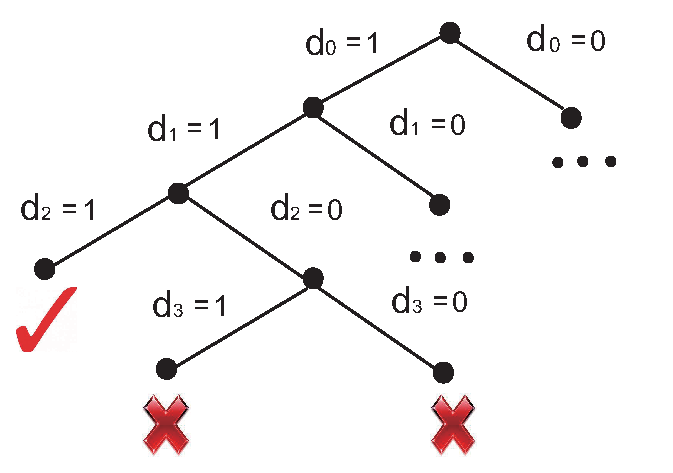
\epsfig{file=figure/search_tree.eps,width=0.6\columnwidth}
\caption{A Snapshot of the Binary Decision Tree with $k=3$}
\label{fig:search_tree}
\end{figure}

\begin{algorithm}[th]
\small
\caption{Argument Conceptualization}
\label{al:backtrack}
\begin{algorithmic}[1]
\Function{AC}{$W, C, L, k$}
\State $\{c_0,...,c_{|C|-1}\}\leftarrow$ Sort concepts $c\in C$ in\ the\ descending\ order\ of $w_v(c)$.
\State $\pi_{max} \leftarrow 0,\pi_{c} \leftarrow 0,ck \leftarrow 0$
\State $d_{max}\leftarrow\{0,...,0\},d\leftarrow\{0,...,0\}$
\State BB($0$)
\If{$ck = k$}
\State \textbf{return} $d_{max}$
\Else
\State \textbf{No solution}
\EndIf
\EndFunction
\Statex
\Function{BB}{$i$}
\If{$i\geq |C|$}
\State \textbf{return}
\EndIf
\If{$ck = k$}
\If{$\pi_{c}>\pi_{max}$}
\State $\pi_{max} \leftarrow \pi_{c}, d_{max} \leftarrow d$
\EndIf
\State \textbf{return}
\EndIf
\If{ISCLIQUE($L,i$) $= TRUE$ and BOUND($i$)$>\pi_{max}$}
\State $ck \leftarrow ck+1, \pi_{c} \leftarrow \pi_{c}+ws_v(c_i), d_i \leftarrow 1$
\State BB($i+1$)
\State $ck \leftarrow ck-1, \pi_{c} \leftarrow \pi_{c}-ws_v(c_i), d_i \leftarrow 0$
\EndIf
\If{BOUND($i+1$) $> \pi_{max}$}
\State $d_i \leftarrow 0$
\State BB($i+1$)
\EndIf
\State \textbf{return}
\EndFunction
\Statex
\Function{ISCLIQUE}{$L, i$}
\For{$j$ from $0$ to $i-1$}
\If{$d_j = 1$}
\If{$(c_i, c_j)\not\in L$ and $(c_j, c_i)\not\in L$}
\State \textbf{return} $FALSE$
\EndIf
\EndIf
\EndFor
\State \textbf{return} $TRUE$
\EndFunction
\Statex
\Function{BOUND}{$i$}
\State $b \leftarrow \pi_{c}$
\For{$j$ from $i$ to $\min\{i+k-ck-1, |C|-1\}$}
\State $b \leftarrow b+ws_v(c_{j})$
\EndFor
\State \textbf{return} $b$
\EndFunction
\end{algorithmic}
\end{algorithm}

Suppose the partial solution of the first $i$ levels in the tree
are $(d_0, d_1, ..., d_{i-1})$ and
the current best solution has a score (computed by \eqnref{eq:f}).
We use $d_{max}$ and $\pi_{max}$ to store the
best solution and its score found thus far; and use $d$ and $\pi_{c}$ to
represent the current partial solution and its partial score.
Variable $ck$ stands for the number of concepts that have been set to
1 in the current decision path, i.e.,
$ck=\sum_{n=0}^{i-1}d_n.$

The main function BB($i$) searches through the tree in a depth-first manner.
It returns when it reaches the leaf node (Line 11-12) or when it has found a
solution (Line 13-16). If the solution is better than the current best,
the current best solution is updated. The function traverses one
more level to include concept $c_i$ (Line 17-19) if it forms
a clique with the currently chosen concepts (ISCLIQUE function)
and if the maximum possible score with $c_i$ is better than
the current best score (BOUND function).

A crucial optimization in this algorithm is that we first sort
all concepts in $C$ in the descending order of their weighted scores (Line 2).
This allows us to quickly
compute the bound (Line 33-34) in linear time (against $k$), i.e., simply
compute the total score of the next $k-ck$ concepts down the decision
tree hierarchy, rather than sorting all the remaining concepts.

